\chapter{Hardware}
This chapter deals with the internal hardware structure of the system as well as the unity test of the specified blocks.

All the hardware that is self developed is placed onto a PCB that is designed in Ultiboard. 

Modules included on the PCB is:

\begin{itemize}
	\item{Horn}
	\item{Distribution Block}
	\item{Motor Controller Unit}
	\item{Speedometer}
	\item{Interface}
	\item{Motor Controller}
	\item{Measurements}
	\item{SDcard}
	\item{CAN-transceiver}
\end{itemize}

The remaining modules are either in a separate case or delivered by Shell Eco Marathon. 

\section{Joulemeter}
The purpose of this block is to be able to measure the energy consumed by the Propulsion Motor. This block differs from the other blocks in that it is only a part of the system during the Shell Eco-Marathon. As the Joulemeter is property of Shell this documentation will not contain any unity test of the block.

\subsection{Analysis}
According to the SEM rules the Joulemeter must measure the energy delivered from the Battery to the Propulsion Motor. The Joulemeter must therefore be located between the Battery and the Power Control-Block (which in turn is located in the Motor Control System). It is very important that the joulemeter doesn't measure energy which isn't consumed by the motor. Thus the following Energy Supply Diagram can be constructed:

\begin{figure}[H]
	\centering
	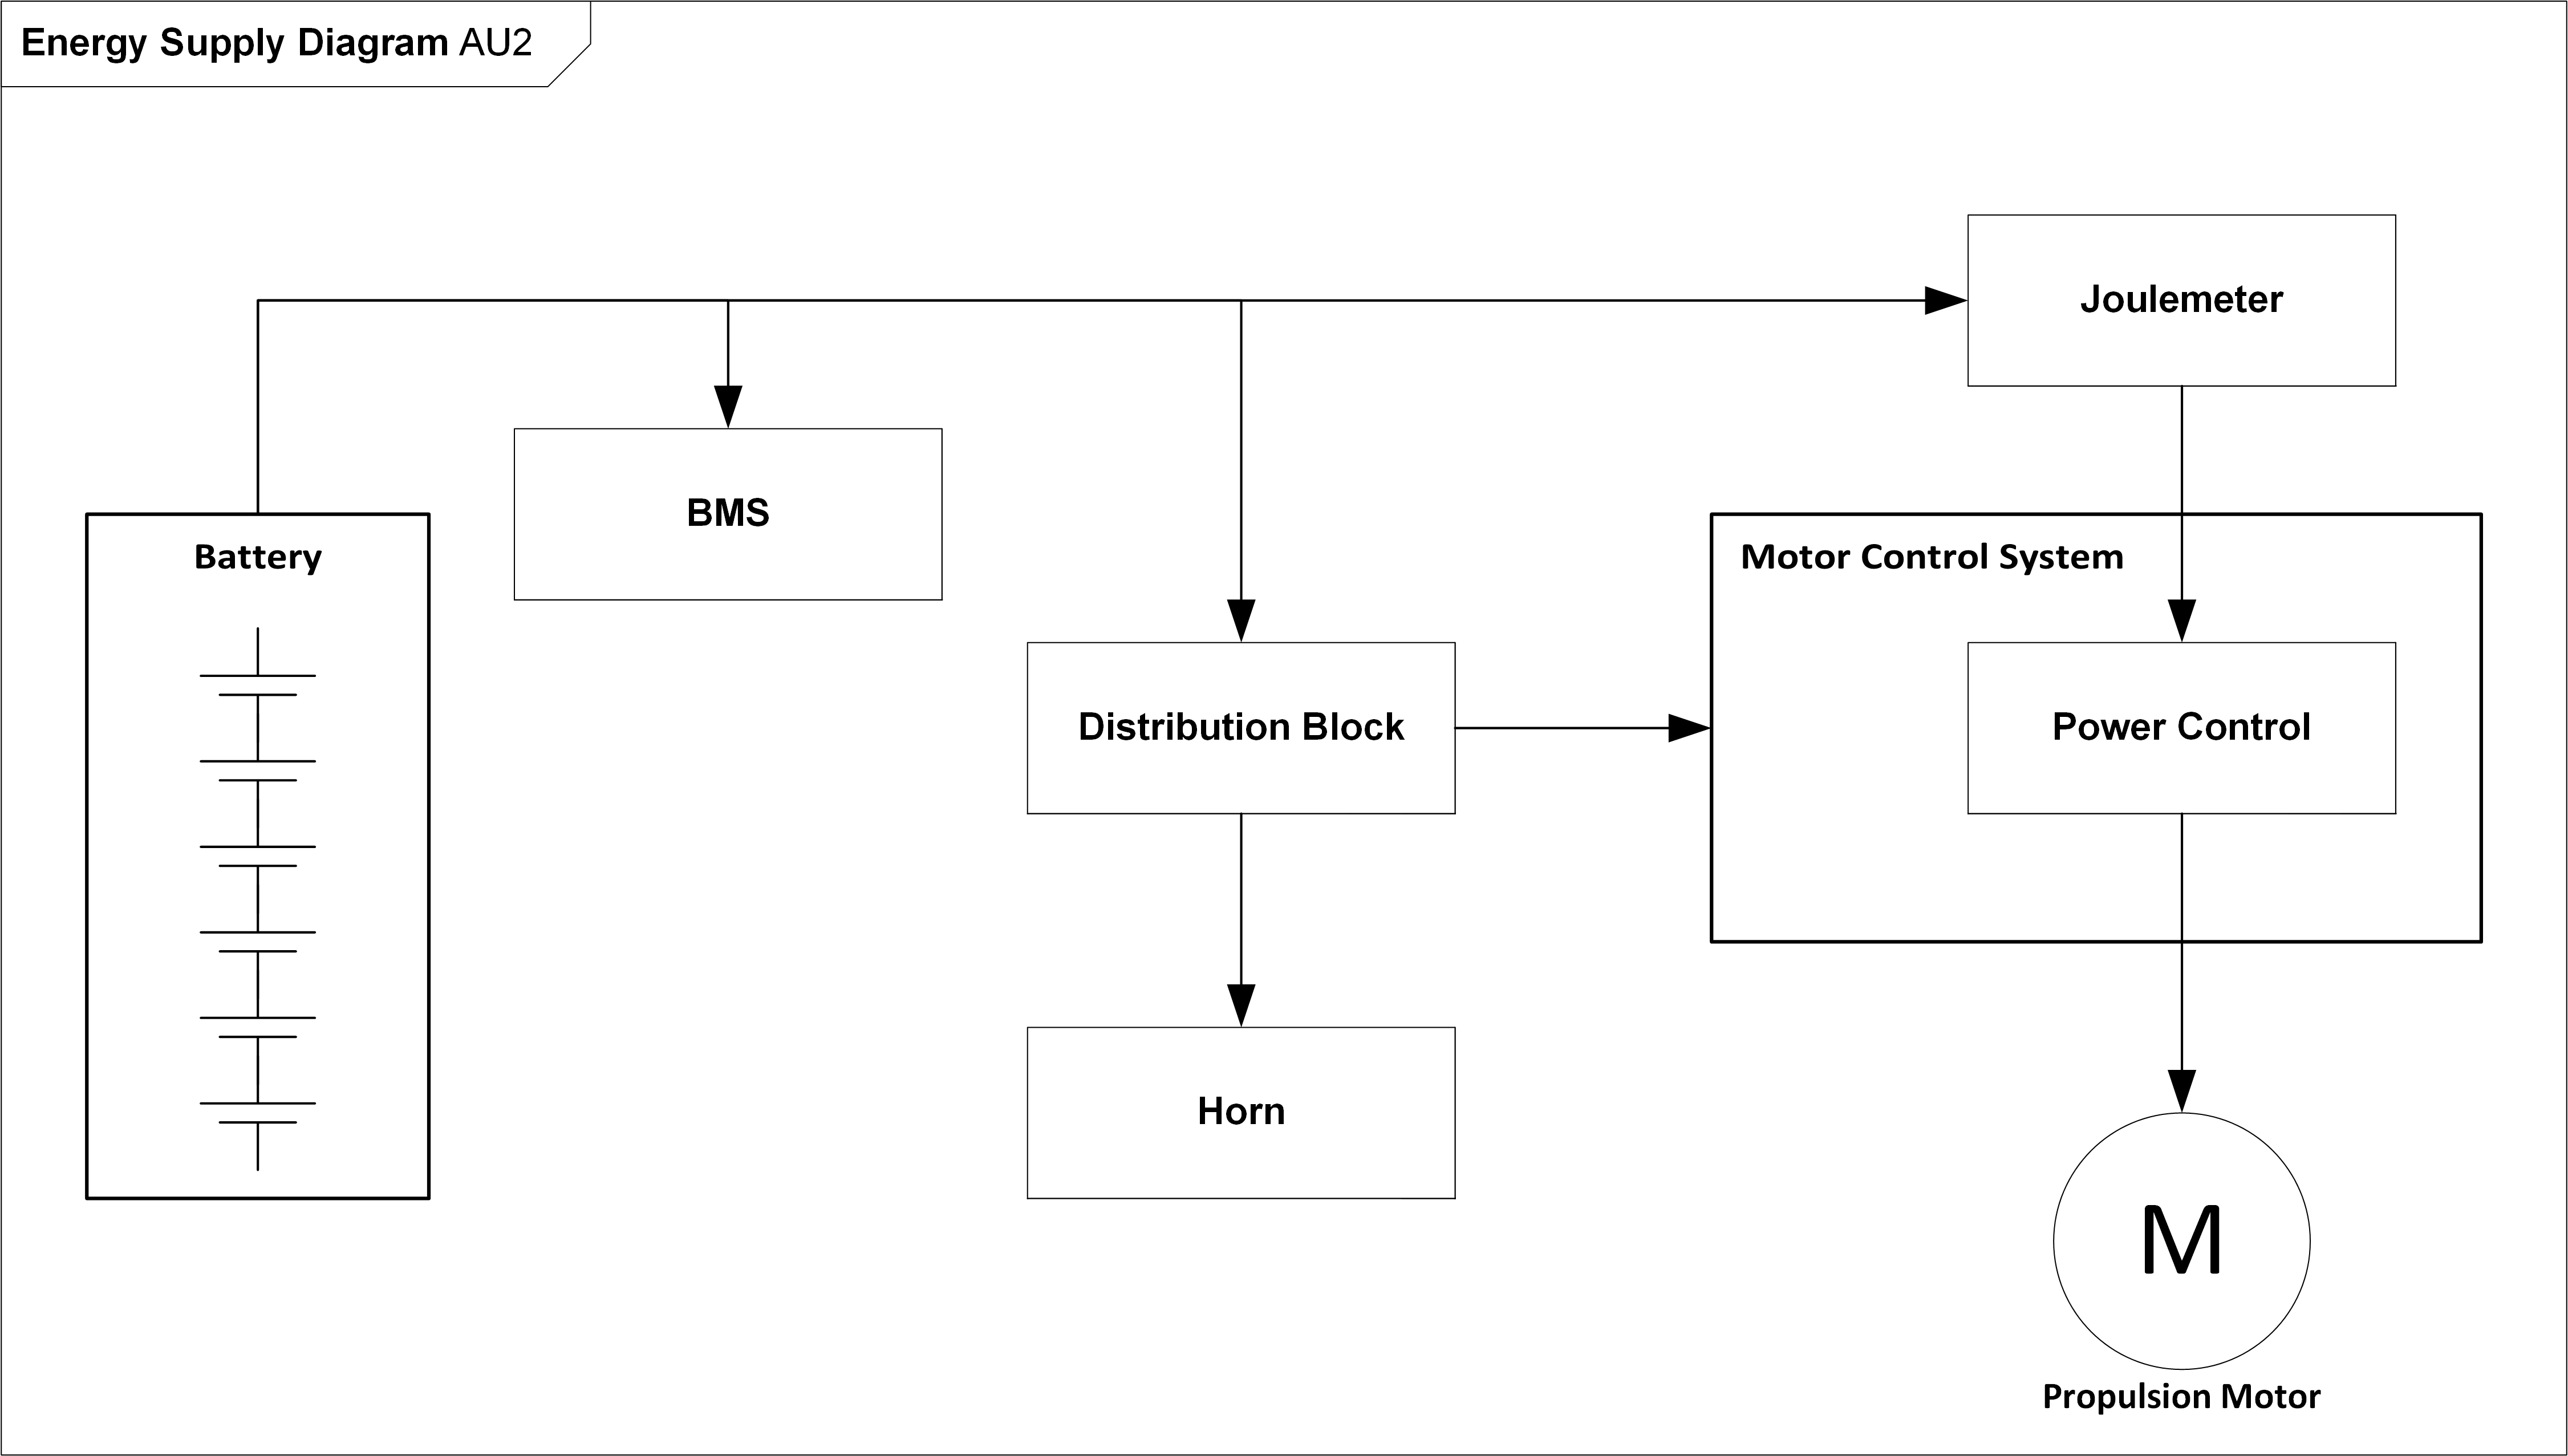
\includegraphics[width=0.9\linewidth]{Hardware/Pictures/Energy_Supply_Diagram}
	\caption{Energy Supply Diagram}
	\label{fig:HAL_application}
\end{figure}

\subsection{Implementation}
The Shell Joulemeter is handed out during the Shell Eco-Marathon and therefore cannot be implemented beforehand. However, according to the SEM requirements the Joulemeter must be located such that the display is visible on the outside of the car. The Joulemeter itself can be implemented by using four spade connectors which can be screwed in place.

When the car is not used to compete in Shell Eco-Marathon the Joulemeter can be disconnected and the Battery can be directly connected to the Power Control Block. It should also be noted that the Joulemeter can be replaced with Rolling Road's Power-sensor - if the user wishes to test the car using the battery.
\section{Battery Management System}
The purpose of the Battery Management System (BMS)...

\subsection{Design}
text

\subsection{Implementation}
text

\subsection{Unity test}
text

\subsection{Debugging}
The purpose of this section is meant to help whoever is going to work with the BMS in the future. Here you will be guided in how to use, debug and program the BMS.

\subsubsection{Programming the BMS}
Firstly, you will need a few prerequisites listed below to be able to program the BMS. Since the BMS was originally build in 2013 the software to program the BMS is outdated but sometimes it is only possible to proceed and get it to work with the specified utilities. 

Tools required to program the BMS are listed here:
	\begin{itemize}
		\item AVR Studio 4 (tested with version 4.19 Build 730).
		\item Atmel Studio 6 or 7 (works with both).
		\item JTAG-ICE programmer	(programmer that is included with the BMS hardware).
		\item 2 batteries to power the BMS (used to power the BMS).
		\item Tera Term (or any other hyperterminal).
		\item USB-A to USB mini cable	(used to debug the BMS and see readouts from Tera Term).
	\end{itemize}


\section{Horn}
The purpose of the horn is to indicate an overtake when coming from behind. The horn is implemented by demand from Shell Eco Marathon. There are various demands that must followed. The most prolific of these is that the horn must emit a sound higher than 85 dB at 4 meters. For other requirements regarding the horn, see section~\ref{sec:requirements}.  

\subsection{Design}
First off, when designing the horn it was necessary to find a suitable horn, that would be able to match the requirements set forth by Shell. There were various options, but it was chosen to use an electric buzzer. This was done as it was the type of horn using the least amount of current. \\
Next up was the design of output stage. In this design it has been chosen to use a BJT transistor. It is used as a switching transistor, turning on and off according to input signal. There is a base resistance which size is defined by the h\textsubscript{fe} and the current used to supply the horn. \\

\begin{align}
	\begin{split}
		I_b &= \frac{I_c}{h_fe}\\
	\end{split}
\end{align}

Lastly, there is going to some safety implemented. Here in the form of a diode, which supplies a path for return current when the transistor is off. This protection is mostly implemented for use with a magnetic buzzer, but it is implemented so that the PCB is prepared for many different kind of buzzers.   

\subsection{Implementation}
A full overview concerning the controls of buzzer can seen on figure underneath.

\begin{figure}[H]
	\centering
	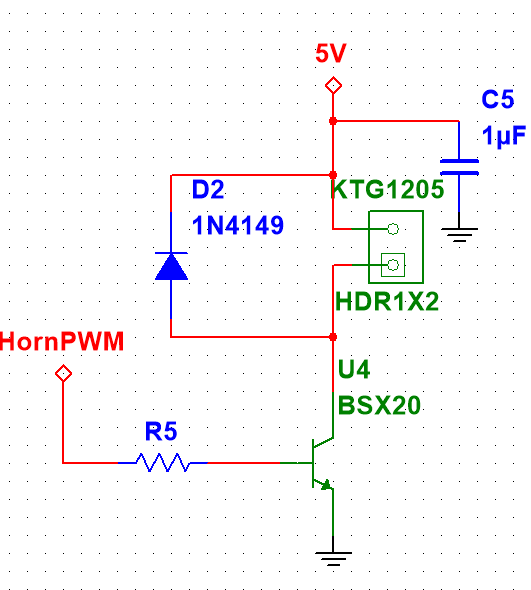
\includegraphics[width=0.7\linewidth]{Hardware/Pictures/Horn_hw}
	\caption{Horn hardware overview}
	\label{fig:Horn control}
\end{figure}

The specific transistor being used is BSX20.

\subsection{Unity test}
text
\section{Distribution block}
A conversion from the 48V to a supply voltage 5V is needed to supply various parts of the circuit. Therefore it is required to use a DC-DC converter for the conversion. It has been chosen by the designer that the converter is being implemented as a switch mode power supply(SMPS from here and onwards). This is chosen as the efficiency of SMPS is increasingly higher than others converters e.g. LDO's. The downside to using a SMPS is additional components must be used.  

\subsection{Design}

When designing SMPS there is several packages out there, that works with passive componentes only. These packages makes the job for the designer much easier as many of the considerations are made for you. Considerations that still much be taken into account are input and output voltages, which already have been decided here. The next thing that can be considered is the efficiency of the package, which is stated in the datasheet.

It has been chosen to use the LT8300 Isolated Flyback Converter from Linear Technology. The implementation is done almost according to the datasheet(see figure \ref{fig:LT8300}) \fxnote{husk ref} except there is implemented a snubbercircuit and a decoupling capacitor before the transformer. Furthermore the values of the resistors are changed.  \\

\begin{figure}[H]
	\centering
	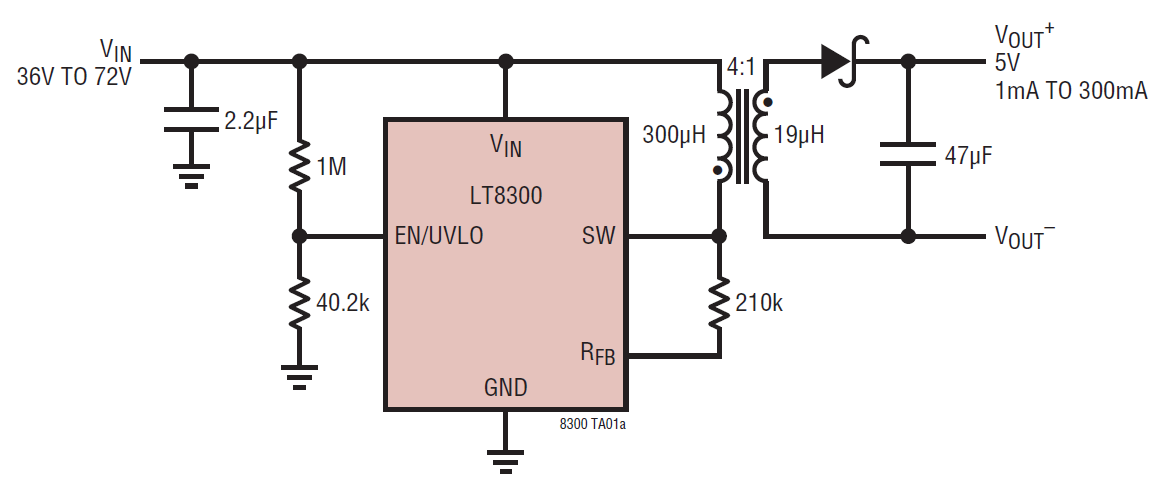
\includegraphics[width=0.6\linewidth]{Hardware/Pictures/LT8300_circuit}
	\caption{Circuit from LT8300 datasheet}
	\label{fig:LT8300}
\end{figure}

\subsection{Implementation}

Figure \ref{fig:SMPS_control} shows the hardware implementation of the SMPS. There is implemented some form of protection circuit before the signal comes into the actual SMPS. This is done by a fuse that limits the current running into the SMPS. 

\begin{figure}[H]
	\centering
	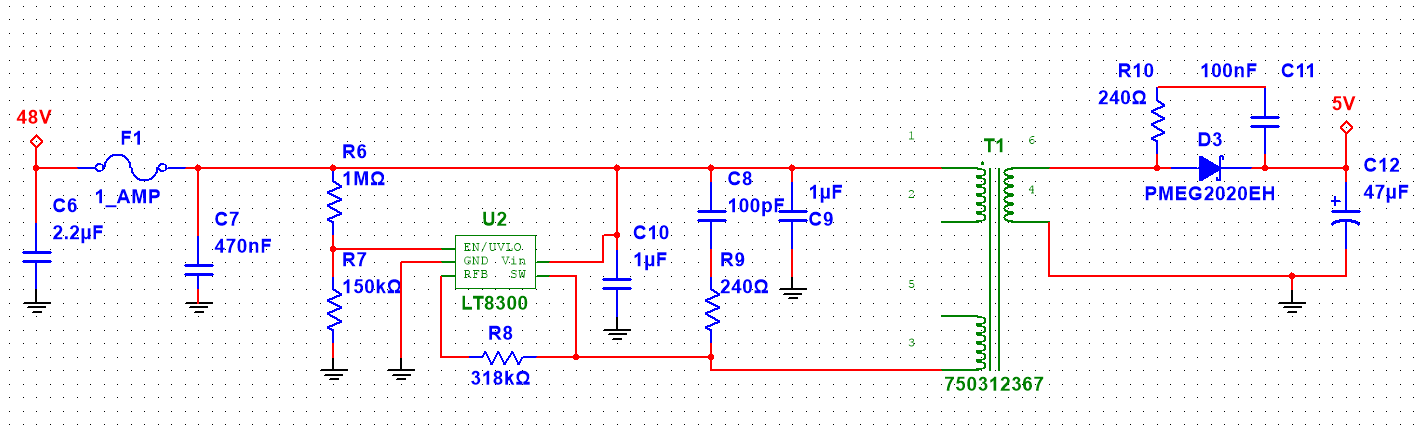
\includegraphics[width=0.7\linewidth]{Hardware/Pictures/SMPS_hw}
	\caption{Step down converter hardware overview}
	\label{fig:SMPS_control}
\end{figure}

There are various resistors can be changed and thereby change the different things e.g. the output voltage. 

The value of the resistor R8 on figure \ref{fig:SMPS_control} is calculated on the formula below. The value of this resistor decides the output of the SMPS.

\begin{align}
	\begin{split}
		R_{FB} &= \frac{N \cdot (V_{out}+V_F)}{\SI{100}{\micro \ampere}}
	\end{split}
\end{align}

Where:\\
N is the number of turns on the primary inductor. Here 6 is used. \\
$V_{out}$ is the desired output voltage from the SMPS. This is chosen to be 5V. \\
$V_F$ is the forward voltage of the diode in output stage. This is set 0.3V as a schottkey is used. \\
$R_{FB}$ is the feedback resistor. \\
This calculation yields a resistance of 318 k$\Omega$.

The dimensions of the snubber circuits are standard sizes. Furthermore, there is used decoupling capacitors to reduce the ripple on the output and to ensure a steady current for the IC.

\subsection{Unity test}
text
\section{Motor Controller Unit}
\label{sec:MCU}
The purpose of the Motor controller unit(MCU) is to implement the motor driving algorithm. It also serves as the logger for the system, receiving data from BMS and logging data onto a SD-card. 

The chosen microprocessor is the PSoC 5LP(low power). This chip is placed onto a prototyping board with the name 'CY8CKIT-059 PSoC5LP Prototyping kit'.\fxnote{Husk ref}

\subsection{Design}

Figure \vref{PSoC} shows the connections associated with MCU. 

The PSoc in use come with a separate programmer, that can be snapped away. There must therefore be implemented an interface to program the PSoC when it is placed onto the PCB. This is realized by the 5x1 HDR as seen on figure \vref{PsoC}.

Capacitor C19 through C21 is capacitors needed by the internal structure of the PSoC. They are setup according to the datasheet and are needed by the ADC's being used. They are bypass capacitors required to ensure proper sampling at high sampling frequencies.

The PSoC is powered by the Distribution Block\vref{SMPS} where it receives 5V. This is within the input limits of the PSoC which ranges from 3.3V to 5V. Here it is being decoupled with a capacitor.  

The remaining connections at use are all the external interfaces to various items the board. This include both inputs and outputs from the PsoC. 

\begin{figure}[H]
	\centering
	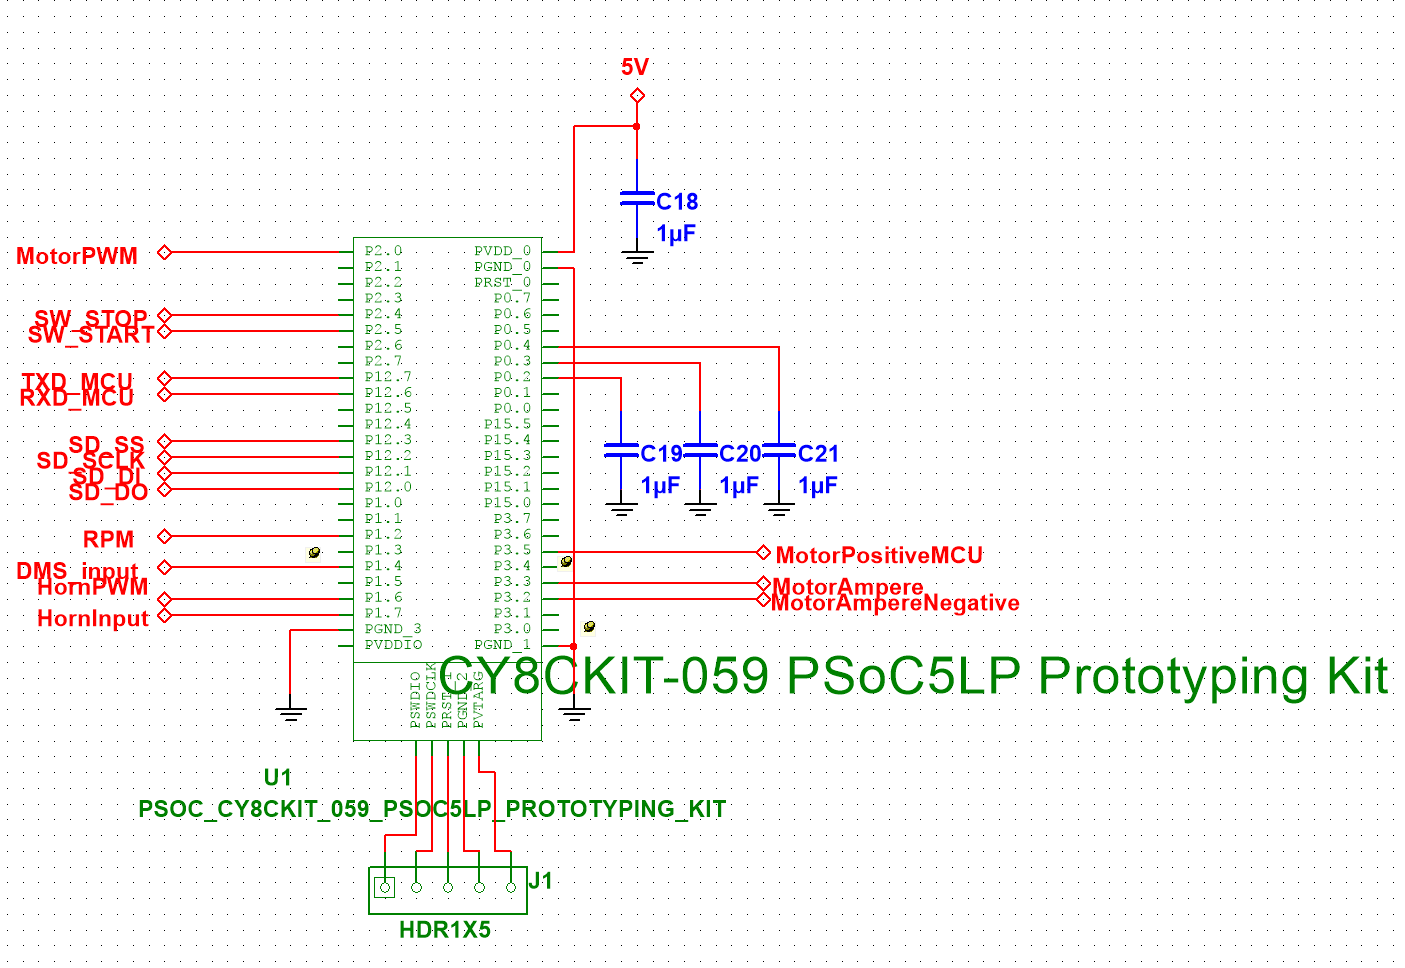
\includegraphics[width=0.7\linewidth]{Hardware/Pictures/PSoC}
	\caption{PSoC connections}
	\label{fig:PSoC}
\end{figure}


\newpage
\section{Speedometer}
The purpose of the speedometer is to measure the car's current speed.

\subsection{Design}
The speed is measured using a TLE49X5L Hal sensor\cite{TLE4905}. This sensor has a digital output wich will go HIGH when a magnet is near the sensor. The voltage level for the HIGH output is equal to the supply voltage V\textsubscript{S}. As the sensor's output is to be measured by the PSoC, then a supply 5 V is used.
In order for the sensor to output a digital signal, it must be connected as seen in the circuit in \ref{fig:HAL_application} below.

\begin{figure}[H]
	\centering
	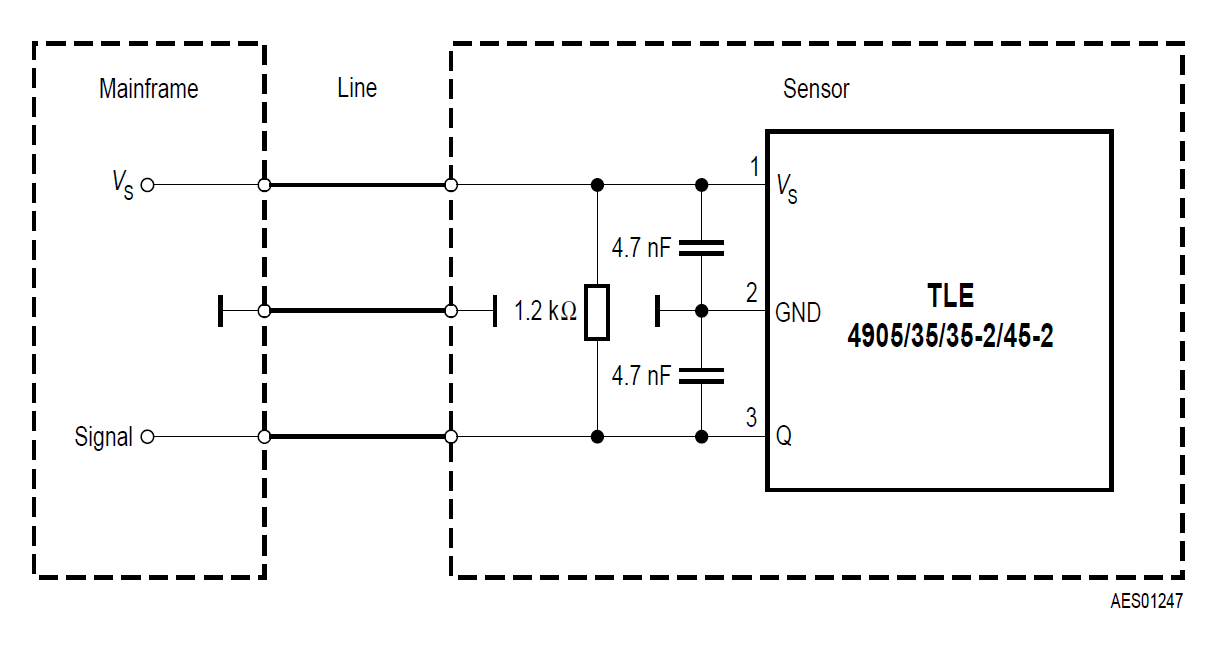
\includegraphics[width=0.6\linewidth]{Hardware/Pictures/HAL_Application}
	\caption{HAL-Sensor application circuit}
	\label{fig:HAL_application}
\end{figure}

The measured objects are magnets \fxnote{name of magnet} which are applied to each spoke of the car's wheel. By placing the sensor near the wheel, then the output signal can be used to measure the speed. A sketch of this configuration is shown in \ref{fig:Speed_sketch} below.

\begin{figure}[H]
	\centering
	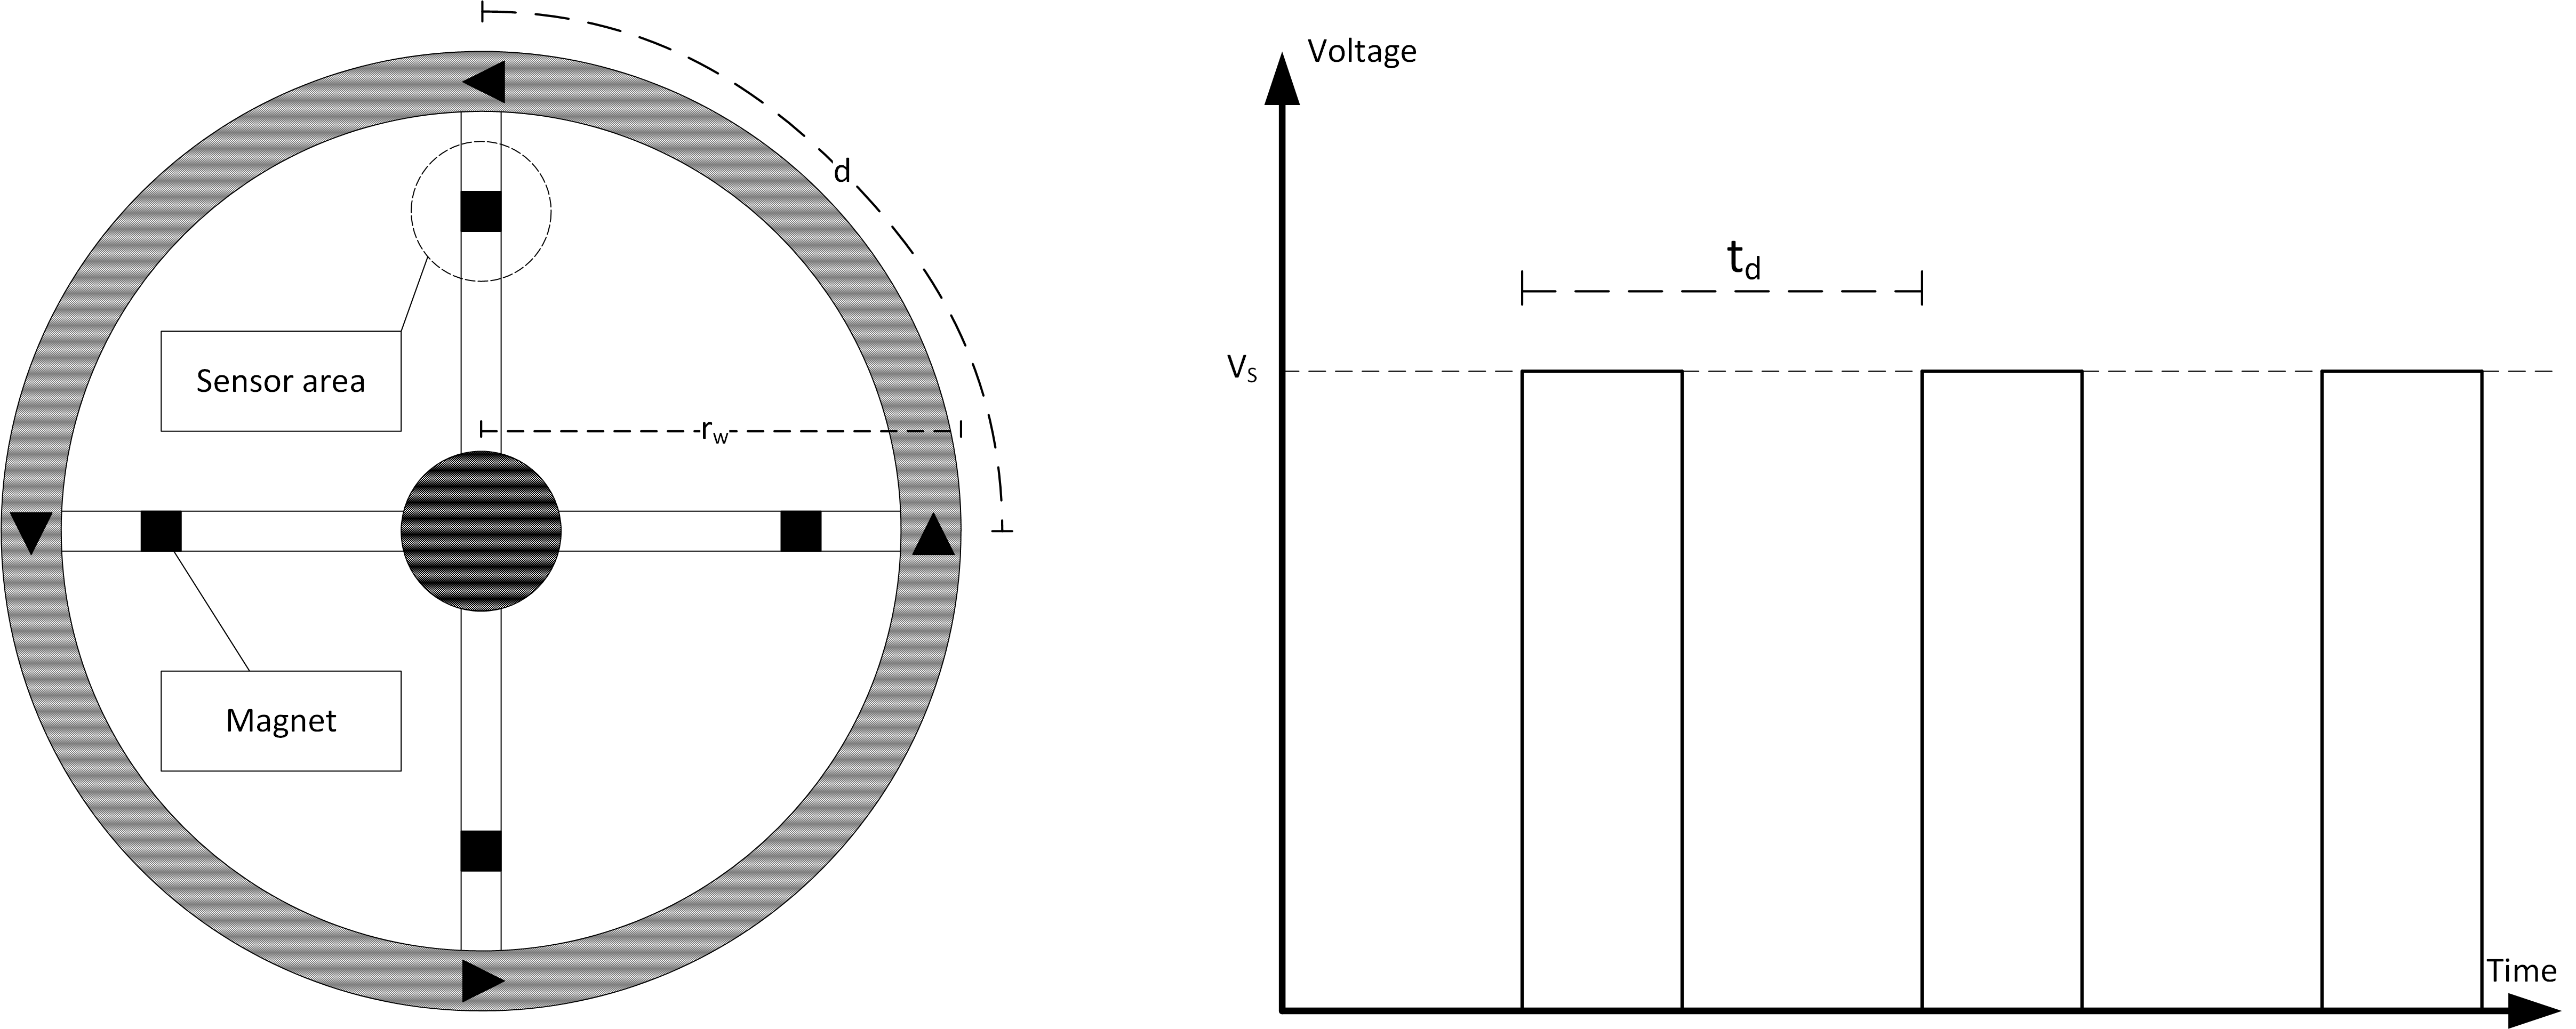
\includegraphics[width=0.9\linewidth]{Hardware/Pictures/Speedometer_Sketch}
	\caption{Speedometer sketch \& sensor output}
	\label{fig:Speed_sketch}
\end{figure}

\newpage
The distance between the rising-edges on the signal is inverse proportional with the car's speed. The distance between each spoke d can be calculated using the wheel's radius r and the number of spokes k on the wheel:
\begin{align}
		d = \frac{2 \cdot r_w \cdot \pi}{k}
\end{align}
This means that during the time between the rising-edges t\textsubscript{d}, the car must have travelled the distance d - if it is assumed that there is no slip between the wheel and the road.\\
The car's velocity v can therefore be calculated as:
\begin{align}
		v &= \frac{d}{t_d}
\end{align}

Neither of the calculations above are completed as the mechanical parts of AU2 wasn't complete during the writing of this documentation. This also results in the fact that the Speedometer hasn't been implemented nor tested. It is, however, the hope that the system can quickly be implemented when the mechanical parts are finished - and that the the speed can be calculated by the PSoC on the fly. 
\newpage
\section{Interface}
The interface gives the user, here the driver, an opportunity to coomunicate with the system. This gives the driver some form of control over the operation of the vehicle. Furthermore it ensures the driver has the ability to use the horn and to keep the dead man safety switch activated as stated by the requirements.

The interface also includes the  connections to the CAN transceiver and the SDcard interface but these will be discussed in their own respective paragraphs accordingly.  
\subsection{Design}

The design consist of 2 connections for each button, with at pulldown resistor at each pin. This ensures no perception of a false positive at the MCU. As seen on the picture, the interface consists of 4 different buttons. These buttons are:

\begin{itemize}
	\item{Dead Man Safety Switch}
	\item{Start button for driving algorithm}
	\item{Stop button for driving algorithm}
	\item{Input for horn}
\end{itemize}

\begin{figure}[H]
	\centering
	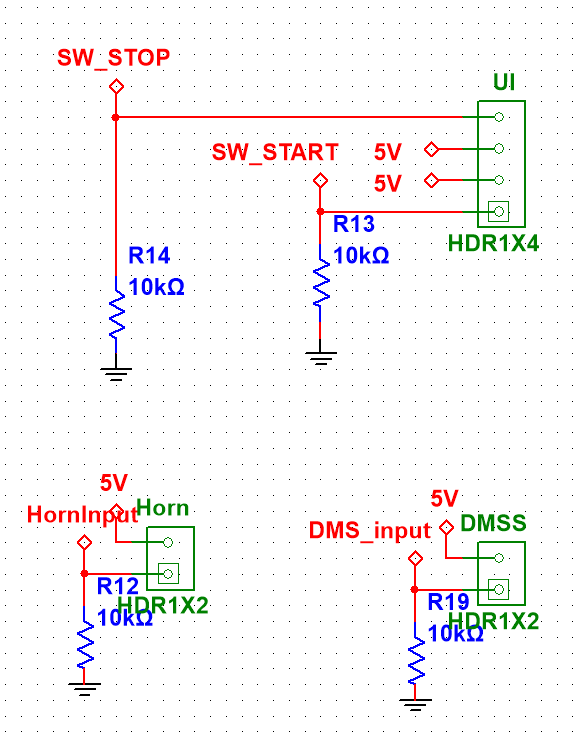
\includegraphics[width=0.6\linewidth]{Hardware/Pictures/User_interface}
	\caption{Interface circuit diagram}
	\label{fig:interface}
\end{figure}

\newpage
\subsection{Implementation}
The buttons will be placed inside the cockpit, which gives driver easy access to them. Since the requirements states that all electronic must be placed behind bulkhead, there must be run long wires from the casing to the buttons. The long wires are prone to noise induction, but this part have been overlooked. This can be done, since the signal running along the wires do not carry sensitive information in the sense that the MCU is indifferent of the voltage level as long as it upholds the limits of MCU.

There hasn't been any final decisions made for which buttons that is going to be implemented into the car to work as the interface. The demands for the button are not high and therefore the choice is open and is depedent on the amount of space given by the engineers building the car.

\subsection{Unity test}
The test is performed by placing the scope on either pin that is connected to a button. Measuring at these points yields a result as shown on the figure \fxnote{Husk at indsætte billede}.

As seen on the figure \fxnote{Husk ref} the measurement equals a step input with minor ripple due to bouncing of the button, which is removed internally in the MCU. 
\section{Motorcontoller}
The purpose of the Motorcontroller is to adjust the speed of the vehicle. In this design it is done by a PWM-signal and a MOSFET. It is of the utmost importance that the hardware affects the motor in the least possible way and thereby affecting the efficiency of the motor itself.

Aside from controlling the motor, this circuitry also senses the voltage and current consumption of the motor. This data is going to the PSoC and is here analyzed. There is, amongst other things, an overcurrent protection built in, to secure the PCB. For more information on this subject see \vref{sec:measurements}.

\subsection{Design}
There are several design considerations to take into account when designing this motorcontroller. The primary and most important feature to this design is the MOSFET that is used. Furthermore the resistor placed between the driver and the MOSFET, decides the amount of current going into the MOSFET and by that how fast it switches(more on this later). On figure \vref{fig:Motorcontroller} it is dubbed 'R18'. 

The figure below(\vref{fig:Motorcontroller}) shows a snippet of the motorcontroller. The parts left out are the measurements as discussed in \vref{sec:measurements}.

There are three components at use here:

\begin{itemize}
	\item{IRFB7530 = Power MOSFET}
	\item{MBR20200CT = Power Diode}
	\item{MCP1407 = MOSFET Driver}
\end{itemize}

The design considerations when using these specific components will be discussed here. Furthermore the components specific application purpose will be mentioned. Lastly, it will be explained as to why this component was chosen.  

\textbf{IRFB7530} \cite{IRFB7530}\\
When using a MOSFET to control a DC-motor, there are numerous precautions that must be taken into account. Most of the precautions will be mentioned further down, when designing the MOSFET driver. 

The MOSFET is the most wide-spread and reckoned way to control a DC-motor and therefore it is chosen here as well. Since the car is not required to run in reverse, it is implemented as a single component and not a H-bridge. This eases the implementation greatly.

This specific component is chosen as it consist of a very low on resistance and thereby the power dissipated in the component will be lower than for a similar MOSFET with a higher on resistance. The maximum on resistance, as described by the datasheet is mere 2 m$\Omega$. Due to a lower power dissipation the heatshink reqiured by the MOSFET to keep it within its operating range, can be smaller or even obsolete. When choosing a MOSFET with a low on resistance, as this is the case, it will come with a very high input capacitance. This is caused by the manufactoring proces of a MOSFET and the values are inversely proportional with each other. For this reason also it has been chosen to implement a MOSFET driver. 

The chosen MOSFET is overdimensioned for this purpose, as it can both endure a much higher current and voltage, than what the motor will operate at. This is done, as the stress that it will be put under during the race will be great and a breakdown would be more or less catastrophic. The specifications can be seen on the table in figure \vref{fig:MOSFET}.

The chosen MOSFET is in the TO-200 housing. This housing is chosen, so that if it is needed to mount the MOSFET on a heat sink it can be done conveniently.  

\begin{figure}[H]
	\centering
	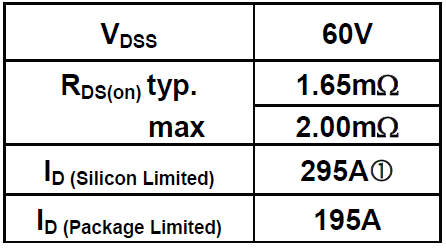
\includegraphics[width=0.85\linewidth]{Hardware/Pictures/MOSFET}
	\caption{MOSFET specifications}
	\label{fig:MOSFET}
\end{figure}

\textbf{MBR20200CT} \cite{MBR20200}

This diode is a flyback diode, in place to secure a known passage for the generated current by the motor, when the MOSFET is shut off. When the motor is supplied is supplied with a current it works as a motor, but when the current is shut off, the motor works as a generator. It is necessary to secure components from possible breaking down after trying to sink the current from the generated motor. The diode is placed in parallel with the motor.

A schottkey diode is chosen for its very fast switching time and less for the low voltage drop. This means that there is a smaller power dissipation in the diode and thereby less loss which equals a higher efficiency. 

This diode is chosen for its specifications to be able to withstand the current coming from the motor. It can be switched with another diode with similar specifications.

\textbf{MCP1407} \cite{MCP1407}

When using a MOSFET driver the design must live up to requirements set forth by the datasheet. This mostly consists of proper placement on the PCB layout, but also includes which capacitors to use as decoupling. But it also leaves a lot for the designer to choose, as there is no suggestions for connections. 

The decoupling capacitors are needed as there is high current requirements for driving the gate capacitance of a standard MOSFET and the IC is therefore in need of a local storage. This also means that the placement of the capacitors must be physically close to the IC to avoid stray capacitances. The capacitors chosen to perform the task, are the same as specified in the datasheet, 1 ceramic and 1 low ESR film capacitor. 

There is connected a resistor to the output pin of the driver. This is included for two reasons. The primary reason being that when using a MOSFET to drive an inductive load, as it is the case here, the di/dt must be reduced as to secure proper switching in the MOSFET. The second reason is to protect the MOSFET, more specific, the gate insultation, which could be damaged by the spikes caused by having an inductive load.

Increasing this resistors value would mean a slower switching time, but would be able to provide a more stable output and decrease ringing. The ringing is caused by the gate being in series with, albeit involuntarily, a small inductor caused by the PCB trace. By decreasing the value of the resistor the turn on peaks of the drain pin increases as well as the ringing. But it also increases the switching time, which makes it a trade off, and causes it to be a major point of optimization in the system. The only boundary for the resistor is that it must be of a certain value to ensure that the components in use doesn't go up in flames.   

The main reason for the choosing to use a driver for the MOSFET is that the PSoC only can deliver so much current. And since faster switching times, means less power loss in the MOSFET which is favorable for when designing a energy efficient vehicle. The argument could be made that the driver also consumes current, but the maximum current drawn from the driver at any time is 150 $\mu $A for typical values. With those numbers the benefits are set to outway the costs.  

This component was chosen as it was already implemented in the Rolling road design and therefore the group had both experience and spare parts of this. This component is easily interchangeable with other components of the same specifications. 

\begin{figure}[H]
	\centering
	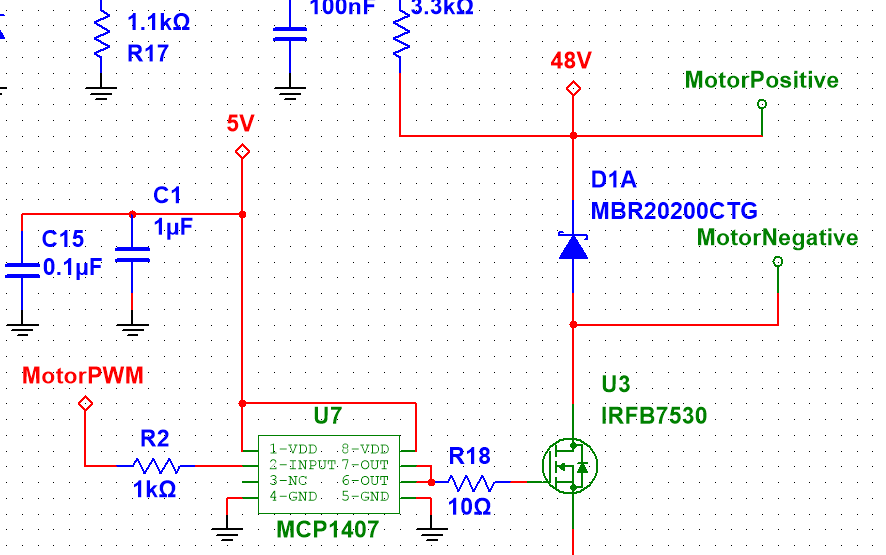
\includegraphics[width=0.85\linewidth]{Hardware/Pictures/Motorstyring}
	\caption{Motor controller hardware}
	\label{fig:Motorcontroller}
\end{figure}


\subsection{Unity test}
There is going to be conducted 2 tests for this module. The first test is a unity test that will make sure the general purpose of the circuitry is working as designed. The other test that will be conducted on this module is a stress test, that will simulate an entire run as it will be in London. 

Neither of these tests have been made at hand in, but are fairly straight forward to conduct. 

The first test consist of hooking up the motor and placing a PWM on the input of the MOSFET driver. Also there must be 48V connected and a working distribution block must be available. A succesful test here is composed of a motor that is rotating. 

The second test must contain the same start parameters as the previous test. The difference here is that this test must first of all run at least 45 minutes. This time should be sufficient to ensure that the testing is done for a long enough period that it can safely be stated that the MOSFET and surrounding circuit can withstand the power dissipation. To take the stress test even further it can programmed to run a higher speed or with a higher load. 
\newpage
\section{Voltage and current measurements}
\label{sec:measurements}
These measurements are done for 2 reasons. The first reason being that is the best and most precise way to calculate the power consumed by the motor and thereby paint a picture of the overall current consumption of the system as it is the motor that is responsible for a large part of the current consumption. This information is also useful in calculating the overall efficiency of the motor. The second reason for measuring is that the MCU contains software that will shut down the system if there is drawn excessive amount of current. 

\subsection{Design}
The design is split up so that there is a section for voltage measurement and a section for current measurement.

The current measurement is done via a shunt resistor. There is placed a measurement point on each side of the shuntresistor that feeds this signal into the MCU. Internally in the PSoC the signal is then amplified and measured. The measurement is conducted as a voltage, but since both the resistance and voltage is known the current corresponding can be calculated via Ohm's law.

The voltage measurement consist of 2 terminals. One before and one after the motor. This is done so that a measurement is different from zero when there runs a current through the motor. But since the signal supplied to the motor consists of 48V and the MCU has a maximum input voltage of 5V, the voltage must be reduced. This is done via voltage divider. This is done so that a voltage of 48V is equal to 5V after the voltage divider. This results in the following resistor values:
\begin{align}
	\begin{split}
		5V &= \frac{R}{X+10k\Omega} \cdot 48V
	\end{split}
\end{align}

Solving for R in the above equation yields a resistance of 1163 $\Omega$. Since this value is not realisable, the value is chosen at \SI{1.1}{\kilo \ohm}, since this is the closest value in the E24 resistor values. This yields a maximum voltage of 4.75V \\
Since there is a high probability of high frequency transients being embeddedd onto the signal there is implemented a low pass filter that also works as an anti aliasing filter. The cut off frequency of this filter is calculated based on the formula below.
\begin{align}
	\begin{split}
		500Hz &= \frac{1}{2 \cdot \pi \cdot \SI{100}{\nano \farad} \cdot R} 
	\end{split}
\end{align}

The above calculations yields a resistor with the value of \SI{3.2}{\kilo \ohm}. Again using the E24 resistor values, this gives a resistor with \SI{3.3}{\kilo \ohm}. With this resistor the cut off frequency is lowered a bit, clocking in at 482 Hz.

Lastly the design is made with protection diodes as extra security measures. These ensures that the input-voltage lies in the range from \SI{-0.7}{\volt} to Vdd \SI{-0.7}{\volt}. 

\newpage
\subsection{Implementation}
The resistance of the shunt resistor is calculated using the formula for a voltage-divider:
\begin{align}
	\begin{split}
		R_{shunt} &= \frac{\rho \cdot l}{A}
	\end{split}
\end{align}

Where:\\
$R_{shunt}$ is the resistance of the shunt resistor\\
$\rho$ is the resistivity of the material. Here it is equal to \SI{16.8}{\nano \ohm}m.\\
l is the length of the wire. Here it is equal to 15 cm.\\
A is the area of the wire, which is 0.7mm.

From the following the resistance of the wire can be calculated and used in the calculations for current consumption. The above calculation results in \SI{3.6}{\milli \ohm}.

The implementation of the voltage measurement requires some thinking. The filter that is implemented makes the calculations for the voltage divider not work, since it also has a resistance that affects the calculations. The are more solutions for this. The first and easiest would be to place a buffer between the two circuits consisting of a op amp. The other solution includes finding the resulting impedance of the filter and taking that number into consideration when dong voltage divider. 
\section{SD-card}
The SD-card is responsible for logging data. The data being logged onto the SD-card is both received from the BMS and data internally from the MCU. The data being logged from the BMS is concerning the state of the batteries. The data being logged from the MCU is concerning the power use of the motor.

\subsection{Design}
Through the design phase it was discovered that purchasing a SD-card module online. This was done and there have no use for designing any hardware for this module. 

The only considerations that must be taken into account when communicating with a SD-card, is that it runs off 3.3V and the MCU that is being used is running 5V. This problem has been taken care of by the card.

As seen on figure \vref{SD} the hardware outlay to communicate with the SD-card is very simple. This is because the add-on board does everything. Furthermore, the specific add-on board here used, is only using the data terminals of the SD-card. There is outputs that are not used with this board, which among other things, sets a pin high when there is a card placed in the holder. 

\begin{figure}[H]
	\centering
	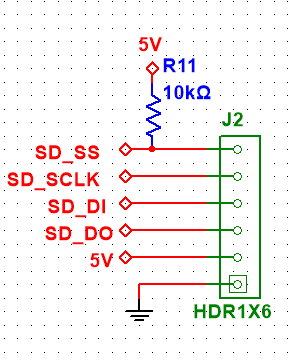
\includegraphics[width=0.7\linewidth]{Hardware/Pictures/SD_card}
	\caption{SD-card schematic}
	\label{fig:SD}
\end{figure}

\subsection{Implementation}
The implementation of the SD-card reader is done away from the PCB. This is done so that reader is removable, in case that it is not needed to collect any data in that specific run and thereby not drawing any, albeit small, current.  

\subsection{Unity test}
The test is done in correlation with the software test. Since it is a board that is bought, it is assumed to work, which the test showed succesfully. 
\newpage
\section{CAN-Transceiver}
\label{sec:CAN-Tranceiver}
The CAN-transceiver is in place to ensure a proper transmission of the CAN signal. Even though the microcrontroller, used as MCU, contains a CAN controller it is still needed to implement a CAN transceiver, according to the protocol as seen on the figure \vref{fig:CAN_Network}.

\begin{figure}[H]
	\centering
	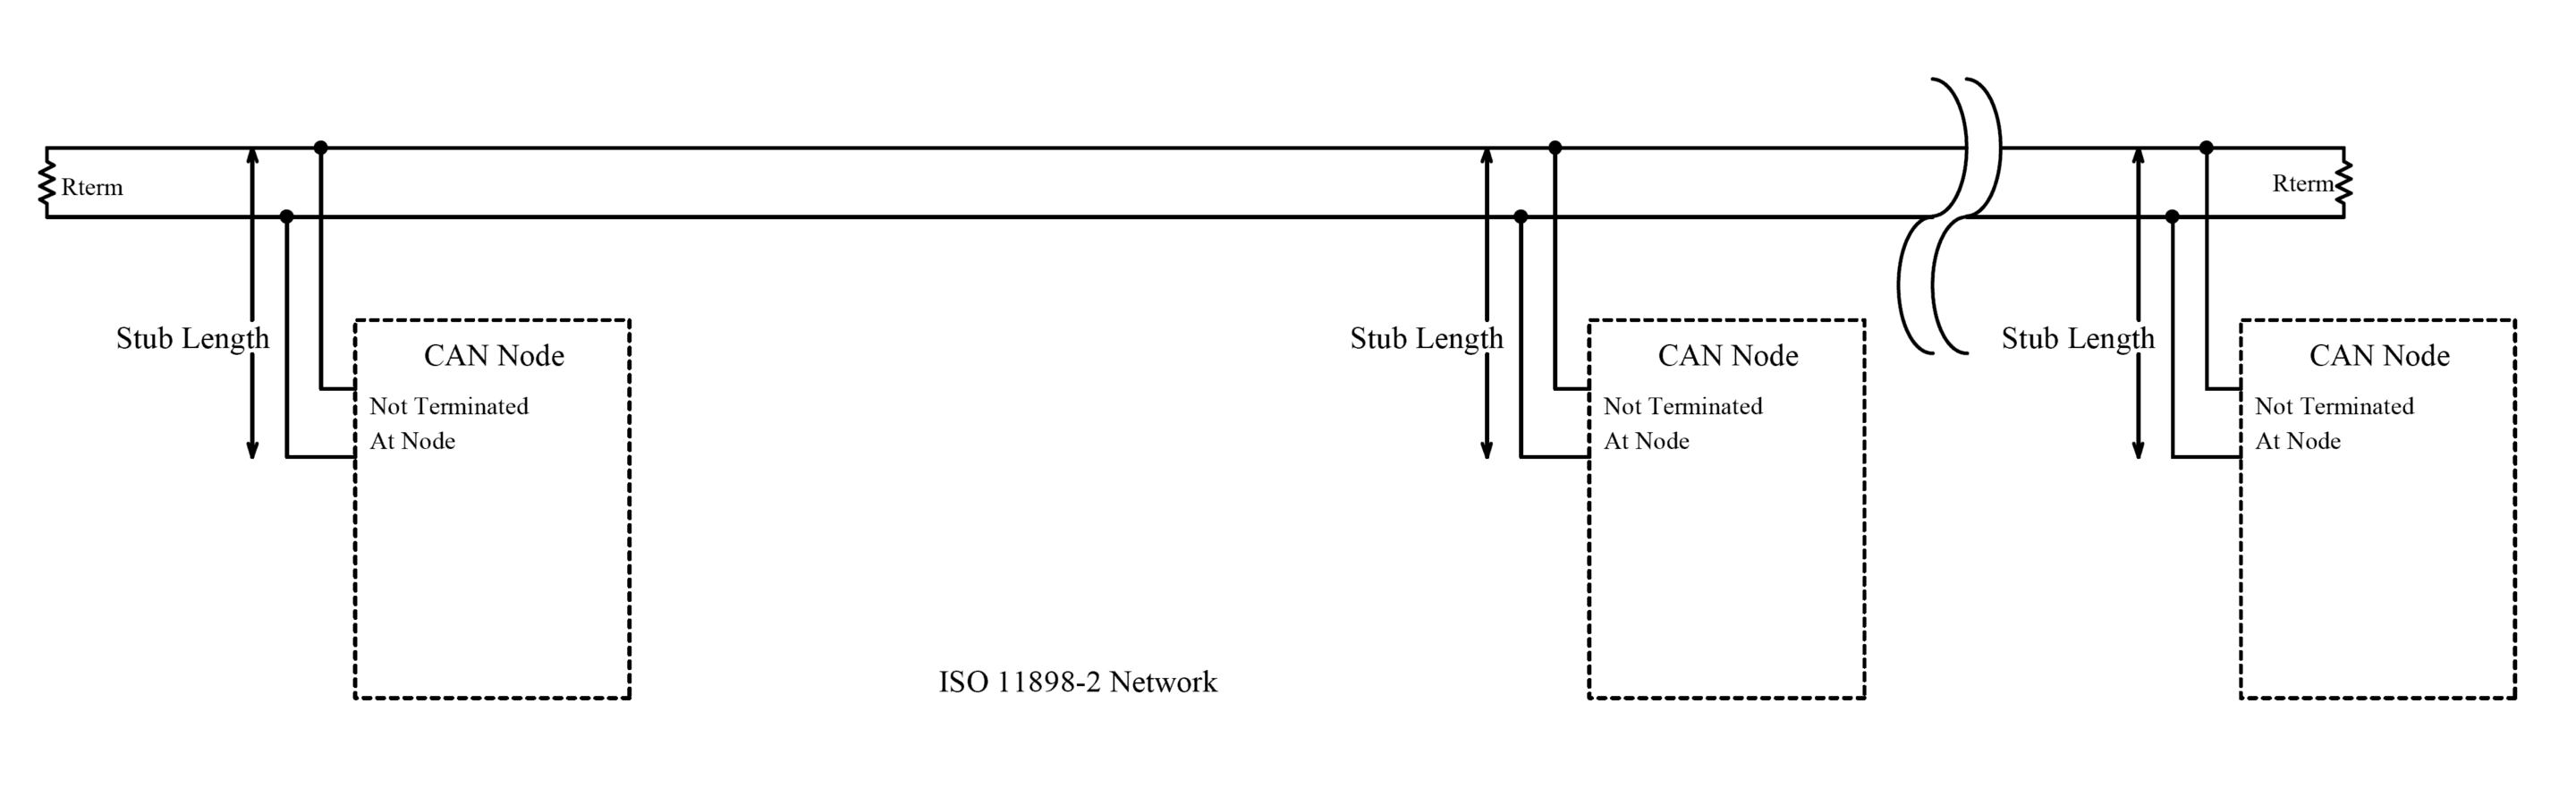
\includegraphics[width=0.7\linewidth]{Hardware/Pictures/CAN_Network}
	\caption{CAN Network overview}
	\label{fig:CAN_Network}
\end{figure}


The CAN bus is used to communicate with BMS and a computer that can be connected to this bus. 

The CAN protocol is implemented, as a result of the BMS in use. On BMS there is implemented a CAN connection and therefore CAN is the obvious choice.    

\subsection{Design}
There exists numerous CAN transceiver packages that can be used for this specific purpose. The specific transceiver at use in this design is SN65HVD1040 \cite{CAN}. This CAN transceiver is chosen for its extremely low power consumption. 

The design for the transceiver can be seen on figure \vref{fig:CAN_hw}. This design is done according to the datasheet. The pin STB is being pulled up with a strong pull up resistor. There is a decoupling capacitor connected on the supply line, as there can occur some relatively large currents as it is a digital circuit. 

\begin{figure}[H]
	\centering
	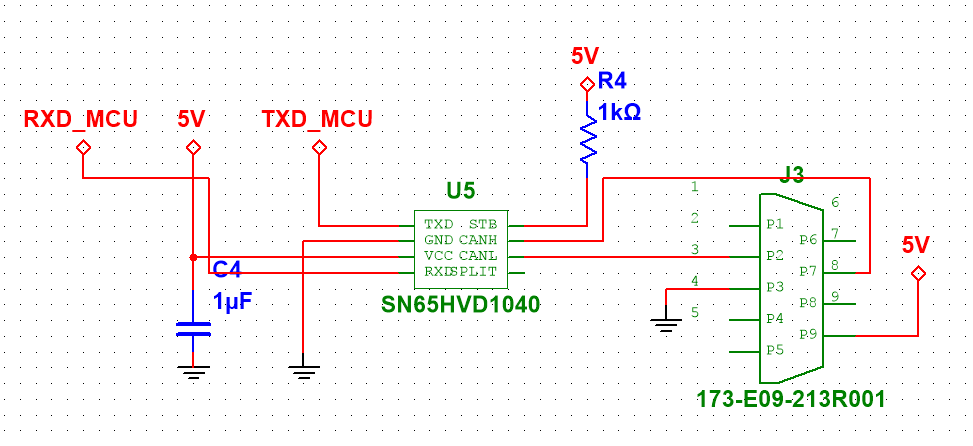
\includegraphics[width=0.7\linewidth]{Hardware/Pictures/CAN_transceiver}
	\caption{CAN transceiver overview}
	\label{fig:CAN_hw}
\end{figure}

\subsection{Implementation}
The implementation is done via a SMD component. Furthermore it is connected to a DSUB9 connector that is used for communication with other systems. The DSUB9 connector is chosen as its counterpart on BMS also uses this connection. The pin-outs are implemented according to the following:

	\begin{itemize}
		\item Pin 2: CAN-low (CAN-)
		\item Pin 3: Ground
		\item Pin 7: CAN-high (CAN+)
		\item Pin 9: Power (5V here)
	\end{itemize} \cite{CAN-Connection}

\subsection{Unity test}
At hand-in this module was not tested. The test can first be done when everything else is up and running as this requires a working PSoC and BMS for it to be properly and thoroughly tested. This is because the rather high complexity of the CAN protocol. 
\section{Propulsion Motor}
Text

\subsection{Design}
text

\subsection{Implementation}
text

\subsection{Unity test}
text